\documentclass[5p,authoryear]{elsarticle}
\usepackage{booktabs}
%\usepackage{enumerate}
%\documentclass{article}

%\usepackage[brazilian]{babel}
\usepackage[utf8]{inputenc}
%\usepackage[T1]{fontenc}

\begin{document}

%
% Autores
%
\title{Learning in Small and Large Ubiquitous Computing Environment}

\author[unisinos]{J.~Barbosa} 
\ead{jbarbosa@unisinos.br}

\author[unisinos]{R.~Hahn} 
\ead{rodrigo.rmh@gmail.com}

\author[unisinos]{A.~Wagner} 
\ead{andre.nho@gmail.com}

\author[unilasalle]{D.N.F.~Barbosa} 
\ead{nice@unilasalle.edu.br}

\author[ufrgs]{C.F.R.~Geyer} 
\ead{geyer@inf.ufrgs.br}

\address[unisinos]{PIPCA/Unisinos, S\~{a}o Leopoldo, RS, Brazil}
\address[unilasalle]{UniLasalle, Canoas, RS, Brazil} 
\address[ufrgs]{UFRGS, Porto Alegre, RS, Brazil}

%
% Abstract
%
\begin{abstract}

GlobalEdu is a generic model created to support learning in ubiquitous
computing environments. This model has the necessary support to implement
learning-related functionalities in ubiquitous environments. The basic
ubiquitous computing support must be supplied by a middleware where GlobalEdu
lays atop. This paper proposes the integration of GlobalEdu with two
middlewares: ISAM and LOCAL. ISAM supports the creation of large-scale
ubiquitous systems. As such, its integration with GlobalEdu results in
large-scale ubiquitous learning environments. On the other hand, LOCAL is
dedicated to create small-scale, location and context-aware ubiquitous
learning environments. The integration between GlobalEdu and LOCAL results in
a local ubiquitous learning system. We created a practical scenario, where our
proposal was evaluated.

\end{abstract}

\maketitle

% TODO - keywords
% TODO - agradecimentos

%
% Introduction
%
\section{Introduction}

Mobile computing is a computational paradigm emerging from wireless networks
and distributed systems technologies. Mobility allows the existence of various
scenarios, from nomadic computing to ubiquitous computing
\citep{weiser91,satyanarayanan01}. In the last scenario, the users, carrying
portable devices (such as handhelds and notebooks) have access to a shared
infrastructure, independently from their physical location or displacement
form. In the viewpoint of ubiquitous computing, the computational power will be
available anytime and everywhere. 

In this scenario, new learning perspectives are essential, due to the
relationship between teaching and learning changes \citep{rogers05}. In our
point of view, a great amount of educational resources will soon be distributed
in a global network, and learning processes will need to explore this diversity
everywhere, anytime and in any device the learners may be employing in their
activities.  Educational applications will explore all the learning
opportunities, joining contextual information (for example, a work of art in a
museum that is being visited) with educational objectives (the learner can be
studying history of art). 

GlobalEdu is a model oriented to ubiquitous learning. It supplies the necessary
support to explore the new learning opportunities available in ubiquitous
environments. GlobalEdu is structured into layers (detailed in section 3) and
can also be coupled with an ubiquitous computing middleware (considered the
third layer). This paper proposes the integration of GlobalEdu with two
middleware projects: ISAM \citep{yamin02,augustin04} and LOCAL
\citep{barbosa07,barbosa08}. The ISAM project focuses on the building and
management of large-scale ubiquitous computing environments \citep{augustin05},
and is being developed at UFRGS (Federal University of Rio Grande do Sul,
Brazil). On the other hand, LOCAL aims to support small-scale,
location-and-context-aware computing environments. It is being developed at
UNISINOS (University of Vale do Rio dos Sinos, Brazil).

% TODO - reorganizar seções
This paper is organized as follows. Section~\ref{sec:ubisupport} presents the
definitions and standards associated with ubiquitous learning.
Section~\ref{sec:globaledu} details GlobalEdu.  Section~\ref{sec:ge-isam-local}
proposes the integration between GlobalEdu and the middleware projects ISAM and
LOCAL. Section~\ref{sec:scenario} describes a practical approach where a
small-scale scenario is being evaluated. Section~\ref{sec:related} compares our
proposal with others in the same area. Finally, Section~\ref{sec:conclusion}
presents some conclusions and plans for future work.

%
% Towards ubiquitous learning support
%
\section{Towards ubiquitous learning support} \label{sec:ubisupport}

Mobile learning (m-learning) \citep{tatar03} is fundamentally about increasing
learners' capability to carry their own learning environment along with them.
M-learning is the natural evolution of e-learning, and has the potential to
make learning even more widely accessible. However, considering the ubiquitous
view, mobile computers are still not embedded in the learners' surrounding
environment, and as such they cannot seamlessly obtain contextual information. 

An ubiquitous learning system \citep{ogata03} can use embedded devices that
communicate mutually to explore the context, and dynamically build models of
their environments. It is considered that while the learner is moving with
his/her mobile device, the system dynamically supports his/her learning by
communicating with embedded computers in the environment. The opportunities
made available by the context can be used to improve the learning experience. 

This learning scenario is attractive, but is not easily implemented. We are
investigating how to better match people's expectations for such a system. In
our point of view, ubiquitous learning environments should support the
execution of context-aware, distributed, mobile, pervasive and adaptative
learning applications. Differently from other research
projects \citep{ogata03,simon03,selene}, the GlobalEdu proposal readily
supports these characteristics. 


%
% GlobalEdu
%
\section{GlobalEdu} \label{sec:globaledu}

GlobalEdu \citep{barbosa05} aims to support ubiquitous educational
applications. Its architecture is based on a layered organization, as shown in
Figure~\ref{fig:ge-arch}. The Application Layer is represented by a
\emph{Pedagogic Agent} (PA), which follows the learner throughout the
environment and helps in her/his interactions with the system.

\begin{figure}[h!] 
  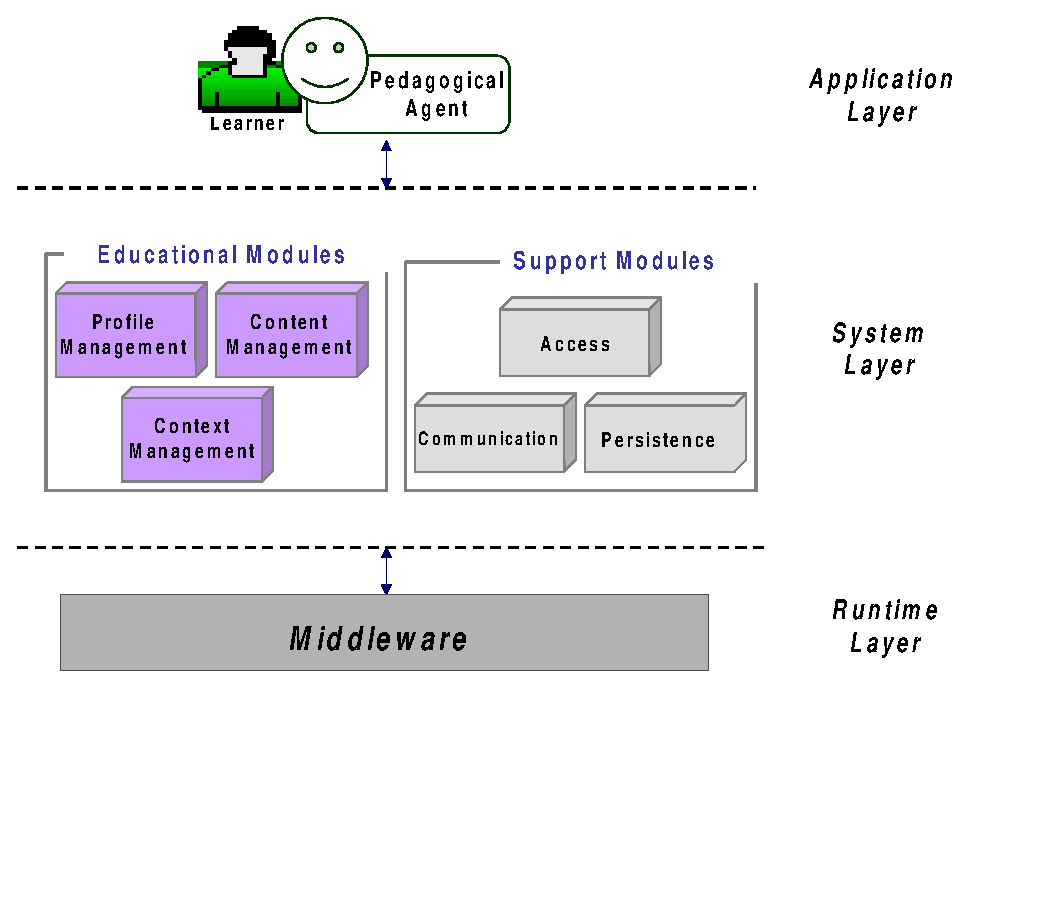
\includegraphics[width=0.5\textwidth]{media/ge-arch}
  \caption{GlobalEdu architecture} 
  \label{fig:ge-arch} 
\end{figure}
  
The \emph{System Layer} is a set of Educational Modules (EM) and Support
Modules (SM).  The Educational Modules are responsible for performing content
management tasks as well as manipulation of the learner model. The system has
three Educational Modules: Profile, Content and Context Management. The first
module is responsible for managing learner profiles. The second one deals with
the learning objects which are manipulated by the learner. The third one
controls information in the context of interest of the learner and is in charge
of adapting the resources that he/she is manipulating. The Support Modules are
intended to help in the execution of the Educational Modules and the
Pedagogical Agent, by managing the aspects of communication, adaptation of
interfaces to devices, user's access and persistence.  

The Runtime Layer is a middleware which supports the execution of educational
applications, providing the system with necessary features, such as perception
of contextual elements, code migration and communication mechanisms.  

For us, one of the characteristics of ubiquitous learning is that the user's
context can be connected with the learner's local context, joining this
information with educational objectives. The \emph{Context Management} module
manages learner context in each location the learner interacts. This module
detects changes of contextual elements in the different locations where the
learner is.  The \emph{Social Context} and \emph{Physical Context} compose the
learner context.  

The \emph{Social Context} has contextualized information about Location Context
and the presence of other PAs in the current context. Location Context contains
information about People (name, e-mail, commitments and roles), Events (type,
description and location) and Resources (name, type, description and
commitments) related to a specific location. The presence of other PAs
presupposes the existence of other learners with the same goals, competencies
and preferences, whose information the learner may access for contact or not.
This information can also be used for the creation of learner groups within the
same context.  

The \emph{Physical Context} represents the resources accessed by the learner,
such as network, locations and devices. We consider that the ubiquitous
computing environment monitors Physical Context elements. Besides, any element
state changes are informed to the \emph{Context Management}.

The \emph{Context Management} module has the capability to know how to locate
the learner in his/her current environment, to identify a learner in the
corresponding context and to provide information adapted to the device the
learner is using. In the same way, each location is modeled as a Geographic
Region and has information about Location Context. So, for GlobalEdu, the
ubiquitous environment is composed by cells and these have different contexts
(Figure~\ref{fig:ge-env}). For example, a University can be considered a cell
and its buildings, different contexts. 

\begin{figure}[h!] 
  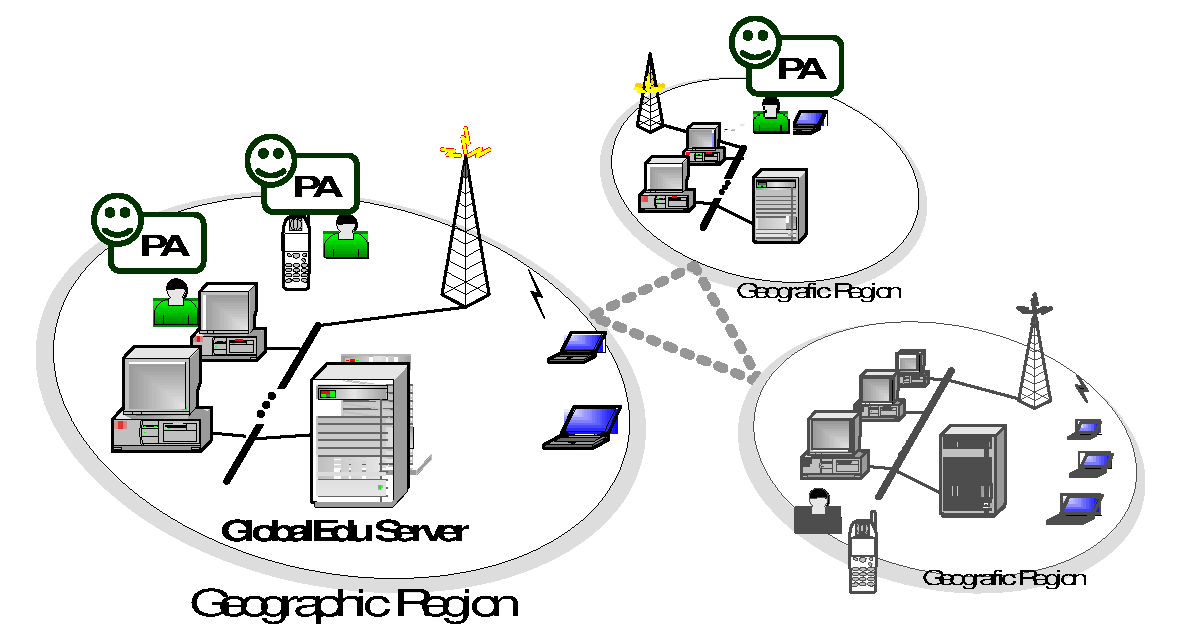
\includegraphics[width=0.5\textwidth]{media/ge-env}
  \caption{The GlobalEdu environment} 
  \label{fig:ge-env}
\end{figure}
  
Learners need to authenticate themselves in order to interact with the
environment. This event is handled by the \emph{Context Management} module.
When a new learner enters into the environment, the Social Context changes. In
this case, the service takes two actions: (1)~notifies other learners in the
corresponding context (Location Context), and (2)~sends to the new learner
adapted information about the current context he/she is in. User profiles are
compared in order to define learners with the same goals, competencies and
preferences, whose information the learner may access for contact or not.  

For the adaptation process, there is a relationship between the \emph{Context
Management} module and the other elements of the architecture (see
Figure~\ref{fig:context-mgmt}). 
  
\begin{figure}[h!] 
  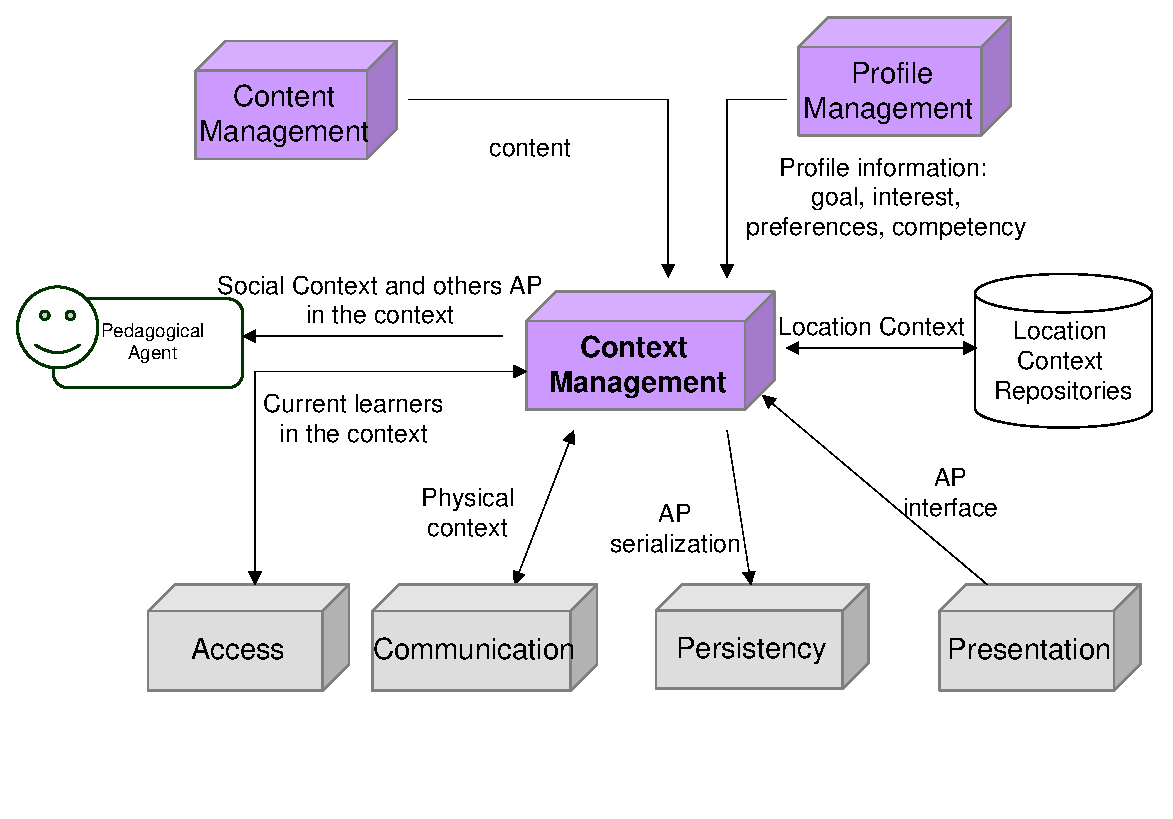
\includegraphics[width=0.5\textwidth]{media/context-mgmt}
  \caption{Context management} 
  \label{fig:context-mgmt} 
\end{figure}
  
With this, learners can ask explicit information about the Social Context they
are part of. He can also extend the search for information to other contexts.
This can be useful in the case of finding learning objects related to the
learner's goals, for instance. 

%
% GlobalEdu, ISAM and LOCAL
%
\section{GlobalEdu, ISAM and LOCAL} \label{sec:ge-isam-local}

GlobalEdu is a generic model created in order to support ubiquitous learning.
This model supports the basic features needed to implement learning-related
functionalities in ubiquitous environments. The basic ubiquitous computing
support must be supplied by a middleware (see Figure~\ref{fig:ge-arch}).
GlobalEdu has been integrated with two ubiquitous environments: ISAM
\citep{yamin02,augustin04} and LOCAL \citep{barbosa07,barbosa08}. ISAM supports
the creation of large-scale ubiquitous systems. As such, its integration with
GlobalEdu results in a large-scale ubiquitous learning system.  On other hand,
LOCAL is dedicated to create small-scale location and context-aware ubiquitous
systems. GlobalEdu integrated with LOCAL results in a local ubiquitous learning
system. 


%
% Large-scale: GlobalEdu and ISAM
%
\subsection{Large-scale: GlobalEdu and ISAM} \label{sec:ge-isam}

The ISAM Project \citep{yamin02,augustin04} provides a common system platform,
allowing the execution of applications across a wide range of equipment as well
as automatic distribution and installation. ISAM is based on the vision that
ubiquitous applications are distributed, mobile and context-aware by nature,
and assumes that ``the computer'' is the whole network (large-scale
pervasiveness). The ISAM Pervasive Environment (ISAM\emph{pe}) is composed of
elements that correspond to the physical infrastructure of the mobile network.
The physical organization adopted in ISAM is the cellular hierarchy (see
Figure~\ref{fig:ge-isam}). Each cell has a base and the cells are connected to
support the ubiquitous environment. A cell manages nodes such as desktops and
mobile devices which can be connected either by wired or wireless networks.

\begin{figure}[h!] 
  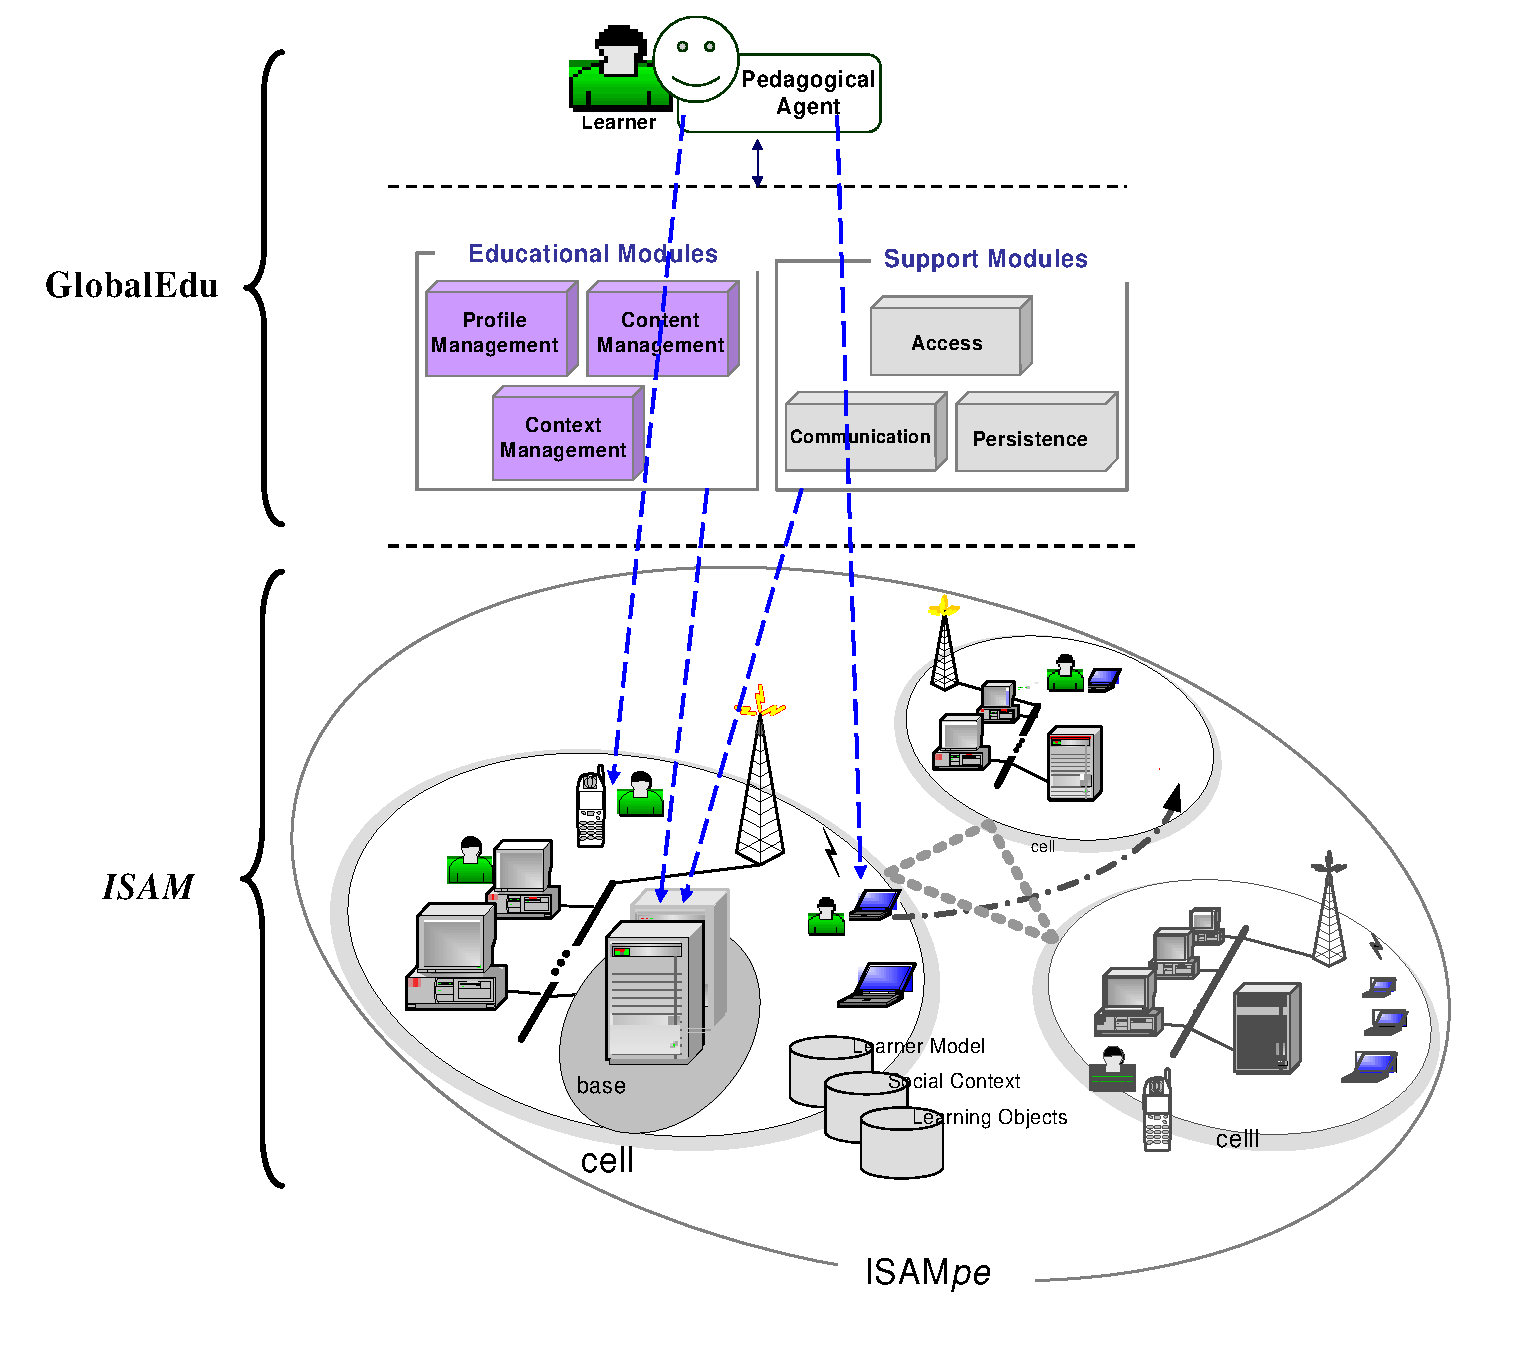
\includegraphics[width=0.5\textwidth]{media/ge-isam}
  \caption{GlobalEdu and ISAM} 
  \label{fig:ge-isam} 
\end{figure}

As can be seen in the Figure~\ref{fig:ge-env}, GlobalEdu also uses a cellular
hierarchy. It is possible to map the GlobalEdu architecture to ISAM (as shown
in Figure~\ref{fig:ge-isam}). The Pedagogical Agent (PA) is mapped to mobile
nodes and the Educational and Support Modules are mapped to the bases (servers
in a cell). The Modules are heavyweight execution units, and are executed in
network servers. On the other hand, PA is a lightweight execution unit, so it
can be executed in mobile devices.

Each ISAM cell has one instance of GlobalEdu. Users can change their context
(cell), carrying their PA. ISAM supports the basic ubiquitous computing-related
aspects and GlobalEdu supports the specific learning aspects.

% TODO
% 
% LOCAL
%
\section{LOCAL}

% TODO... completar...

LOCAL is composed by seven subsystems (see Figure~\ref{fig:local-arch}):

\begin{enumerate}

  \item \emph{User profiles}, which store information related to the learning
        process.

  \item \emph{Personal assistant}, which resides in the user's mobile device. 

  \item \emph{Location system}, used to determine the physical position of the
        mobile equipments.

  \item \emph{Learning objects repository}, which stores and indexes content
        related to the teaching process.

  \item \emph{Tutor}, an analysis engine capable of making inferences by using
        the data supplied by the profiles and the location system. 

  \item \emph{Communication system}, used to establish communication between
        the different parts of LOCAL, and between the system and its users.

  \item \emph{Event system}, used to schedule tasks. The following subsections
        describe these components in detail.

\end{enumerate}

\begin{figure}[h!] 
  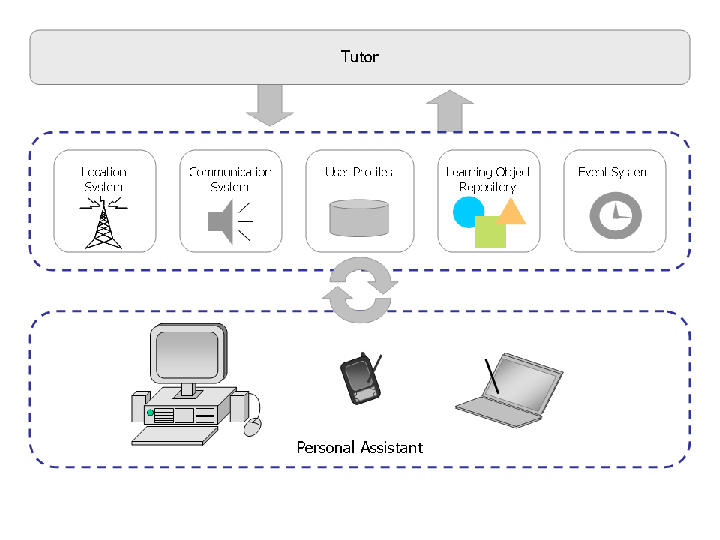
\includegraphics[width=0.5\textwidth]{media/local-arch}
  \caption{The LOCAL architecture}
  \label{fig:local-arch} 
\end{figure}

\subsection{Learner Profiles}

In the last few years, the search for standardization of user profiles has led
to several research efforts like PAPI \citep{papi08} and LIP \citep{lip09}. In
the scope of ubiquitous learning, profiles allow the exploration of resources
based on characteristics of both the learner and the contexts in which he/she
interacts.  This is underlined in \citet{barbosa06}, \citet{ogata03},
\citet{nivo07} and \citet{selene}.

The \emph{user profiles} in LOCAL are based on the PAPI standard. Reasons
behind this decision include: 1)~flexibility -- PAPI can be freely extended,
and all of its components are optional; 2)~modularity -- profile fields and/or
sections can be handled separately, allowing part of the profile to reside in
the \emph{personal assistant}, while another part is tied to the visited
contexts. User profile data can be either persistent or contextual (see
Figure~\ref{fig:profiles}). 

\begin{figure}[h!] 
  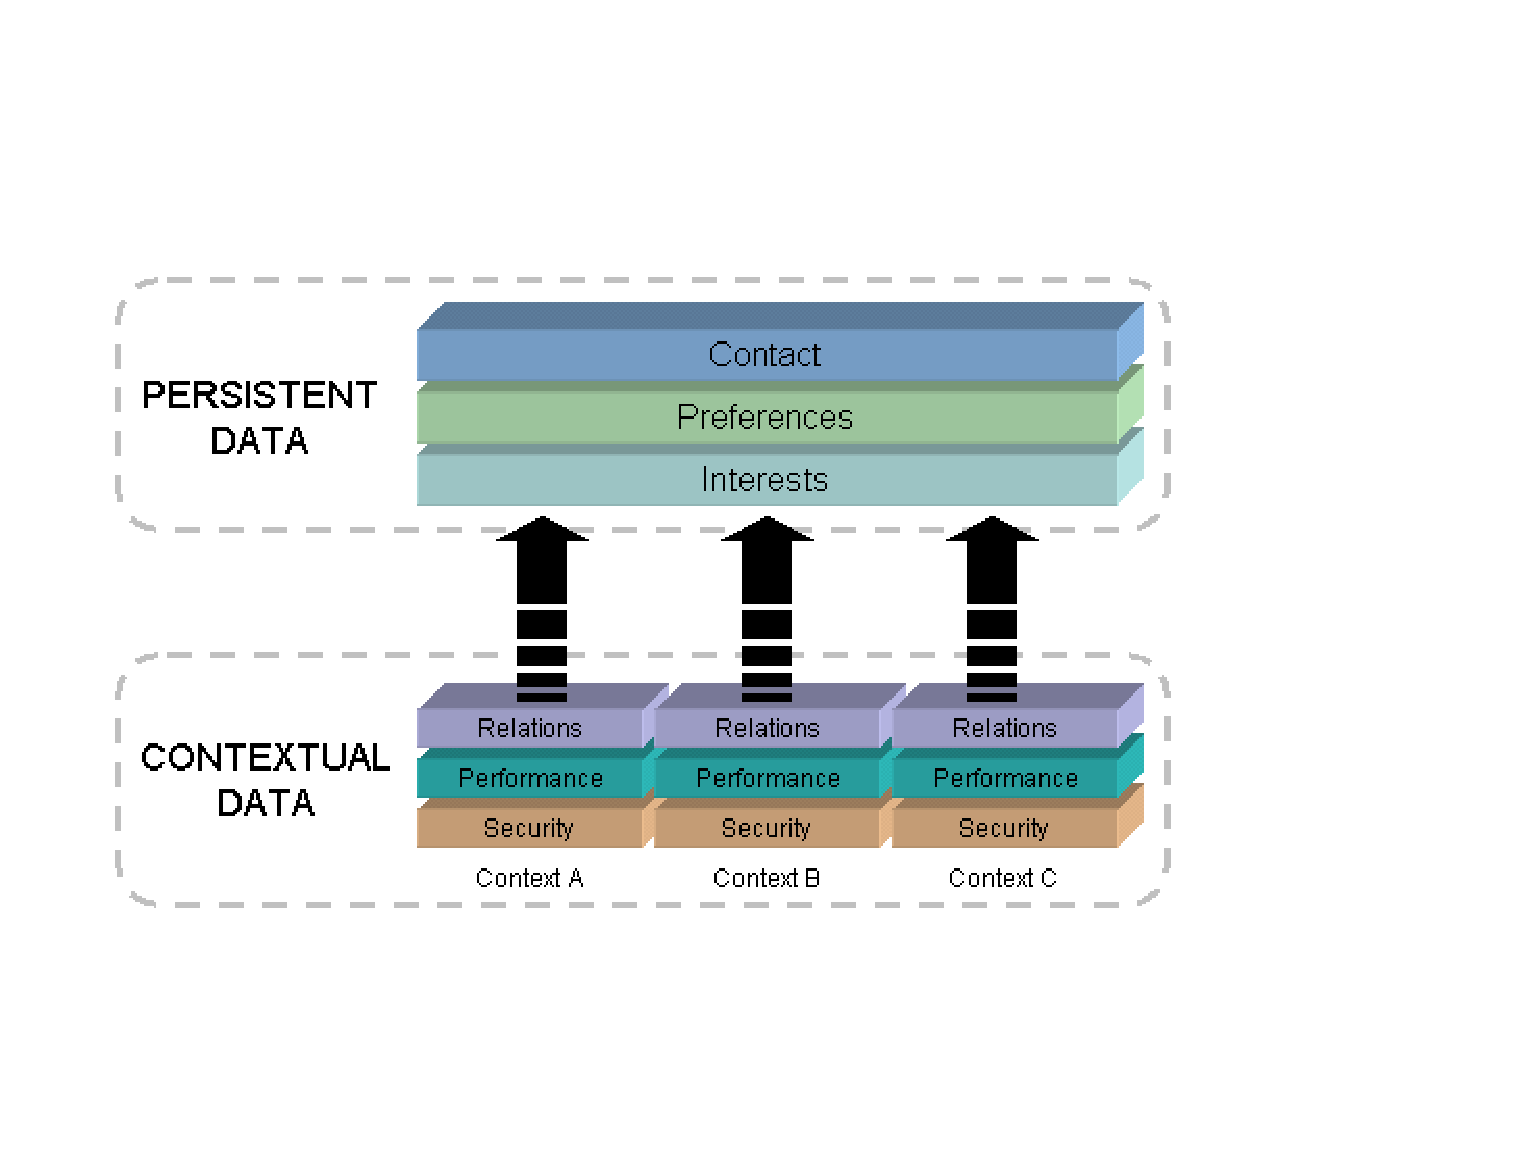
\includegraphics[width=0.5\textwidth]{media/profiles}
  \caption{Organization of learner profiles in LOCAL}
  \label{fig:profiles} 
\end{figure}

The persistent data (\emph{Contact}, \emph{Preferences}, \emph{Interests}) is
stored in the \emph{personal assistant}, and it always accompanies the learner,
no matter which context he/she is in. The contextual data (\emph{Relations},
\emph{Performance}, \emph{Security}) is associated with the many contexts in
which the learner interacts. LOCAL manages both kinds of data, seeking for
pedagogical opportunities. 

\emph{Contact} stores basic user data, such as name, address, e-mail and phone
number.  The \emph{Preferences} section helps the system customize the user
experience, storing configuration data related to the preferred media type
(audio, video and/or text), and others not directly related to pedagogical
activities. Also, the learner might suffer from some kind of physical
disability. In this case, according to specific disability scenarios, the
system can provide the same content in different formats. For example, if the
learners of a particular group are following a video tutorial, a transcript
would be of particular use to people who are hard of hearing. 

The \emph{Interests} section follows the knowledge areas defined in the ACM
Computing Classification System \citep{acm98}, having a general knowledge area
(for example, ``Math'') and a specific interest topic, in the scope of said
knowledge area (for example, ``Group Theory''). The specific areas are then
classified according to the apprentice's own goals (for example, ``to learn''
or ``to teach''). \emph{Relations} stores data which specifies relations
between other users in the same context (for example, ``student'', ``teacher''
or ``researcher''). \emph{Performance} refers to proposed goals and evaluations
conducted in a context. \emph{Security} stores credentials (names and
passwords) to allow for different access levels in specific contexts. 


\subsection{Personal Assistant and Location System}

The \emph{personal assistant} (PA) is the module which accompanies the learner
in its mobile device. It allows users to stay connected to the system, while
providing a certain degree of independence. The PA presents the following
functionalities: 

\begin{enumerate}
  
  \item Authentication, keeping track of the learner's connection status.
  
  \item Access to the location system, allowing for turning it off at will.

  \item Receiving and storing notifications proceeding from the communication
        system.

\end{enumerate}  

The \emph{location} system used by the LOCAL is based on a generic
architecture, supporting different methods of determining user's physical
locations. The system ties physical location data to symbolic names (contexts).
This allows real time mapping of mobile device positions. As the learner
authorizes the location system in its PA, it begins to determine the device's
position and physical context changes, along with the time and date of such
changes. With this data, it is possible to completely track the learner's
movements. User profile data, alongside context information, is used in the
learning process. 



\subsection{Learning Objects}

Learning objects in LOCAL are made available to learners in accordance with
whatever pedagogical opportunities may appear during their interaction with the
different contexts (see Figure~\ref{fig:objects}). The location system keeps
the tutor aware of which context the learner is in (step 1). The tutor uses
this information, as well as the learner's profile data, to select the objects
meeting the learner's goals and the context (steps 2 and 3). The objects
meeting these criteria are then forwarded to the learner (step 4). This
adaptive process can be started by two events: 1)~when the learner enters a new
context or 2)~insertion of new material at the object repository. The metadata
specification for Learning Objects in LOCAL was made in accordance with the
IEEE LTSC \citep{ltsc08}. The ample acceptance of this standard is underlined 
in \citet{rigaux09}.

\begin{figure}[h!]
  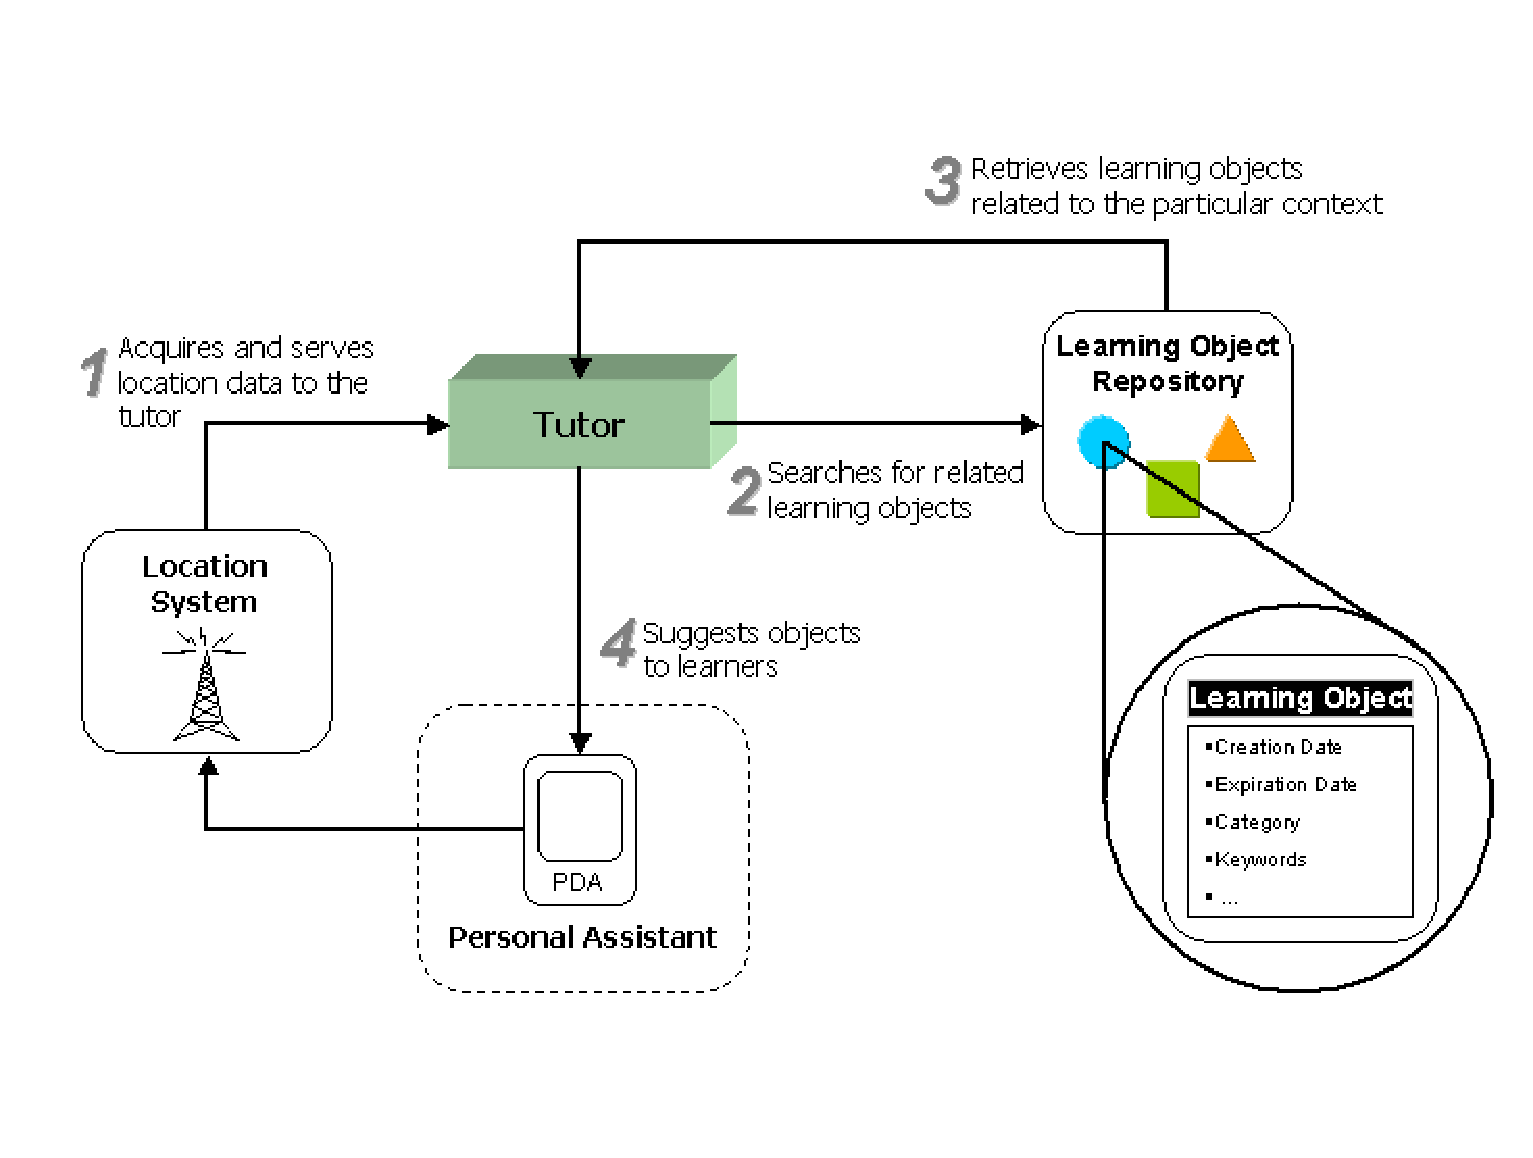
\includegraphics[width=0.5\textwidth]{media/objects}
  \caption{Learning objects management}
  \label{fig:objects} 
\end{figure}



\subsection{Tutor}

The tutor uses profile and location data to find learning opportunities. It can
act in two ways: 1)~sending learning objects (described in the last section)
and 2)~stimulating interaction between learners. It uses learner profile data
to create bonds between learners (see Figure\ref{fig:interaction}). There are two interaction
forms: 1)~\emph{Similar interests}: the tutor finds learners with similar
interests in the same context, and stimulates interaction. This approach can be
used in the creation of workgroups in a classroom, for example;
2)~\emph{Complementary interests}: the tutor finds learners with complementary
interests. For example, a learner who wishes to learn more about a particular
subject is paired along a user who wishes to teach or knows more about it. This
way, the tutor can be used, for example, to create pairs of students who
complement each other.

\begin{figure}[h!]
  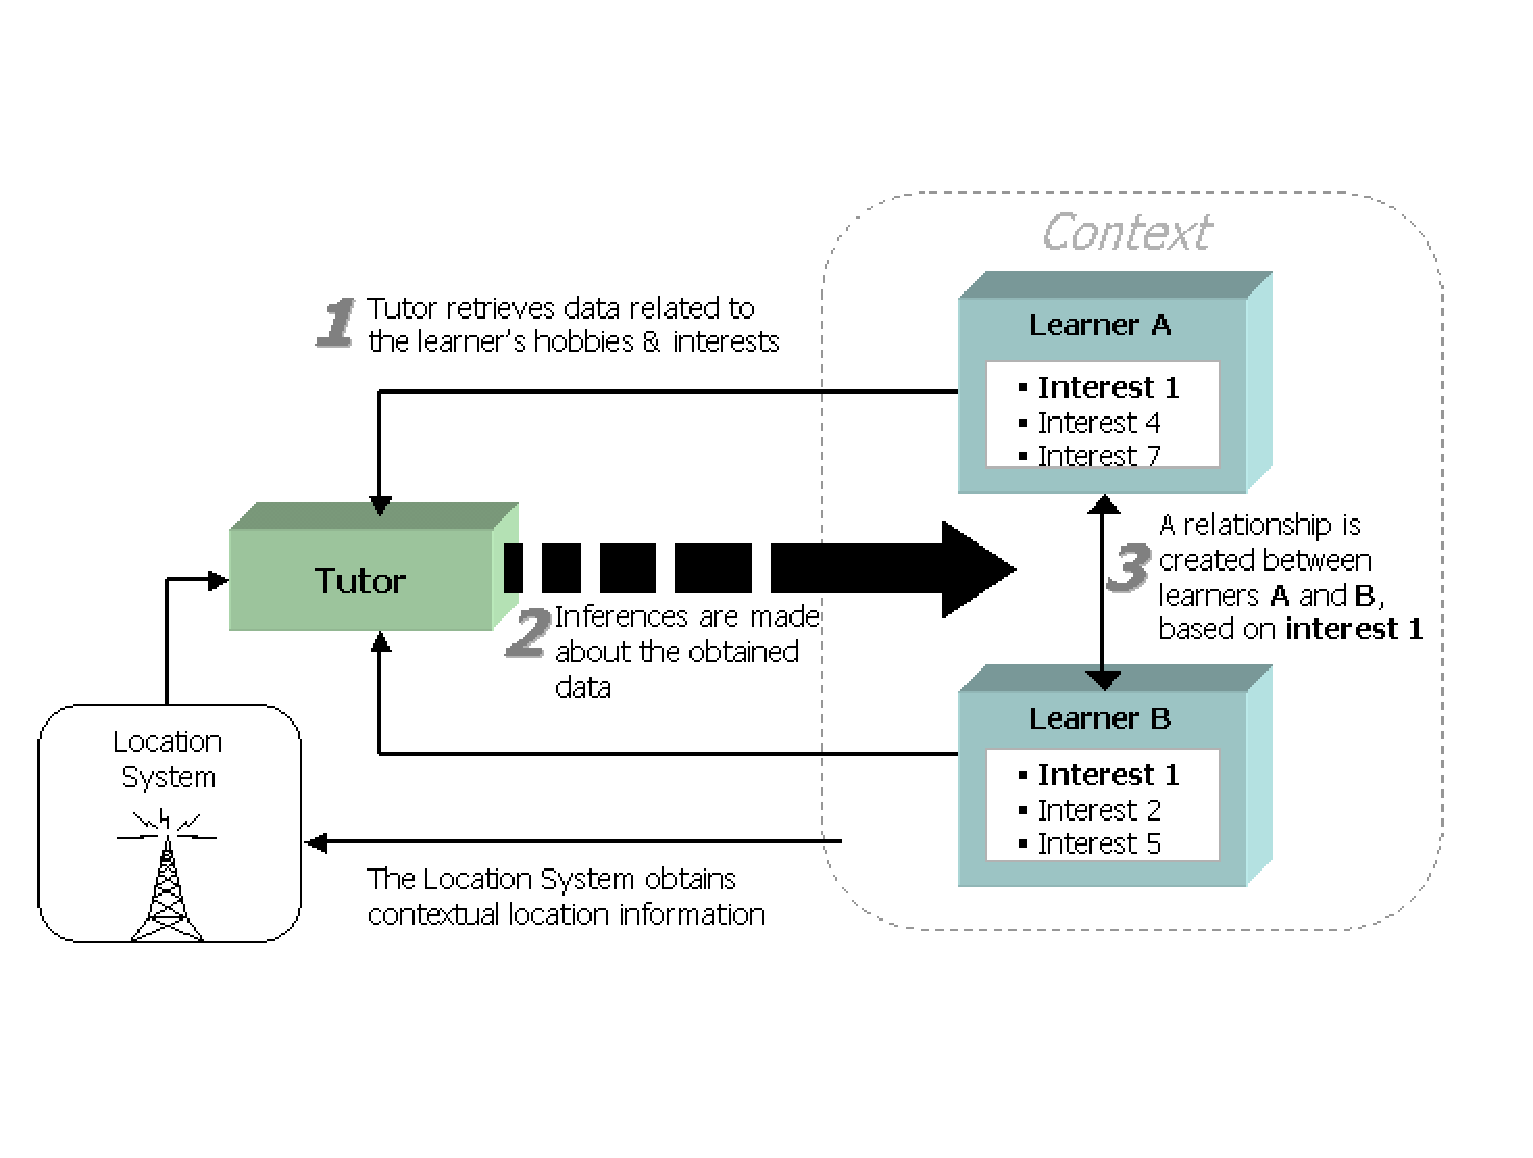
\includegraphics[width=0.5\textwidth]{media/interaction}
  \caption{Organization of learner profiles in LOCAL}
  \label{fig:interaction} 
\end{figure}


\subsection{Communication System \& Events}

The \emph{communication} system present in LOCAL is used to establish contact
with learners, notifying them of new pedagogical opportunities. This system can
be controlled automatically, or by an operator using the administrative
interface.  Users are contacted by textual notifications. The notifications are
sent according to profiles, objects, location and event data. The following
services are supported: 

\begin{enumerate}

  \item Sending messages to a specific user in the system, wherever it is. 

  \item Sending messages to a specific context (everyone in the context
        receives the notification).

  \item Sending messages to a user, but only if he/she is inside a particular
        context.

  \item Sending messages to all users, regardless of context. 

\end{enumerate}

The messages also have an associated date of expiration, delimiting a time
interval after which the message loses its validity.
Figure~\ref{fig:communication} shows an example of use for the communication
system where, based on the location data (1) and user profiles (2A), the tutor
contacts the learner (3). This can be used to presenting new pedagogical
opportunities, for instance. The communication system also supports the
creation of events. An event is characterized by a series of properties,
including keywords, starting date and location. Events can be defined to a
future date, in usual date format (\emph{yyyy-mm-dd hh:mm:ss}) and have an
arbitrary duration. When a message is associated to an event, it is up to the
tutor to find correspondences, and forward the messages at the appropriate
time. 

\begin{figure}[h!]
  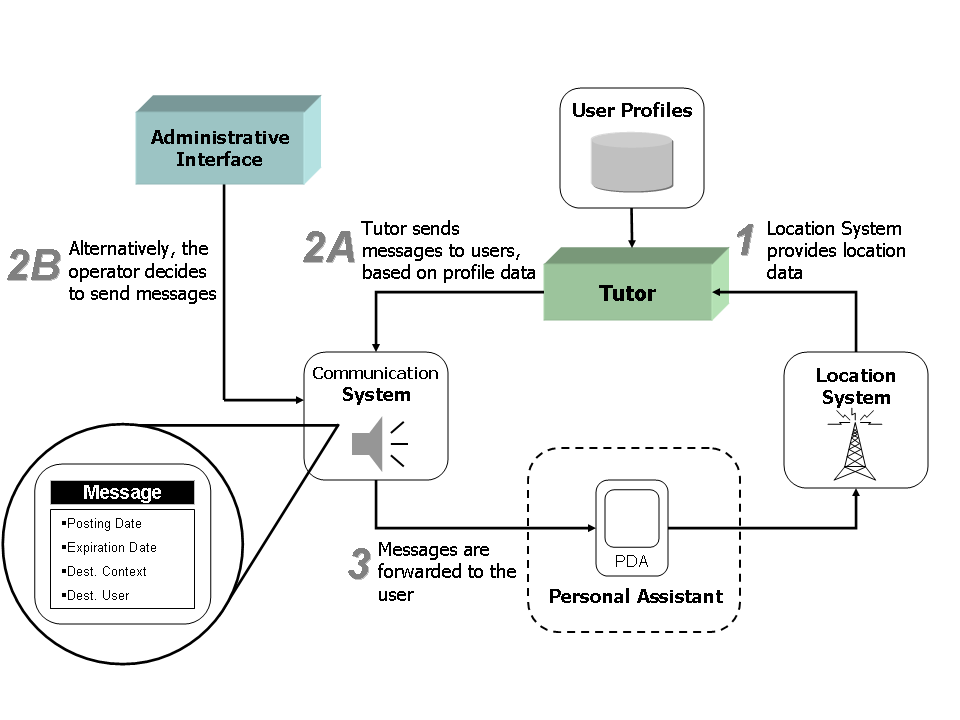
\includegraphics[width=0.5\textwidth]{media/communication}
  \caption{Communication System}
  \label{fig:communication} 
\end{figure}


%
% Small-scale: GlobalEdu and LOCAL
%
\subsection{Small-scale: GlobalEdu and LOCAL} \label{sec:ge-local}

The LOCAL project \citep{barbosa07,barbosa08} aims to provide a
location-and-context-aware ubiquitous architecture geared to create small-scale
learning environments.  LOCAL is composed by seven subsystems (see
Figure~\ref{fig:local-arch}): (1)~\emph{User Profiles}, which store information
related to the users using the PAPI standard \citep{papi08};
(2)~\emph{Personal Assistant}, which acts as the system's interface, residing
in the user's mobile device; (3)~\emph{Location System}, used to determine the
physical position of the mobile devices; (4)~\emph{Learning Objects
Repository}, which stores and indexes content related to the teaching process;
(5)~\emph{Tutor}, an analysis engine capable of making inferences by using the
data supplied by the profiles and the location system; (6)~\emph{Communication
System}, used to establish communication between the different parts of LOCAL,
and between the system and its users; (7)~\emph{Event System}, used to schedule
tasks. 

\begin{figure}[h!] 
  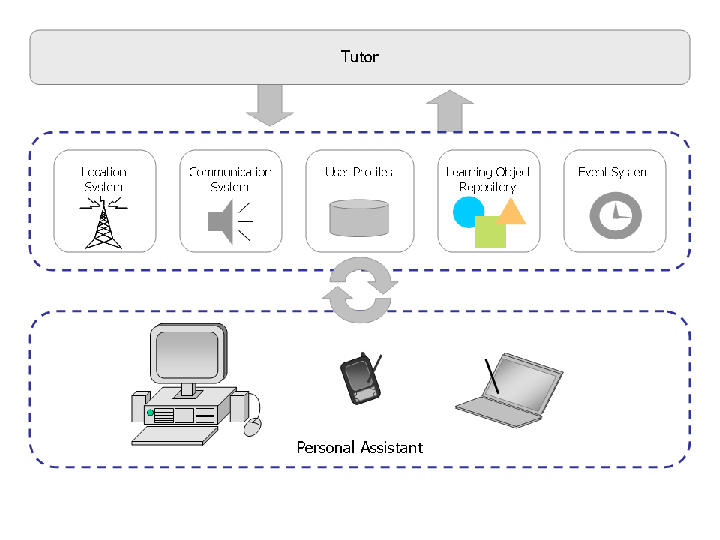
\includegraphics[width=0.5\textwidth]{media/local-arch}
  \caption{The LOCAL architecture} 
  \label{fig:local-arch} 
\end{figure}
  
The \emph{personal assistant} (PA) is the module which accompanies the learner
in its mobile device. It allows users to stay connected to the system, while
providing a certain degree of independence. The \emph{location system} ties
users' physical location data to symbolic names (contexts). This allows real
time mapping of mobile device positions.  As the learner authorizes the
location system in its PA, it begins to determine the device's position and
physical context changes, along with the time and date of such changes. With
this data, it is possible to completely track the learner's movements. User
profile data, alongside context information, is used in the learning process.
  
\emph{Learning objects} in LOCAL are made available to learners in accordance
with whatever pedagogical opportunities may appear during their interaction
with the different contexts. The location system keeps the tutor aware of which
context the learner is in. The tutor uses this information, as well as the
learner's profile data, to select the objects meeting the learner's goals and
the context. The objects meeting these criteria are then forwarded to the
learner.  The metadata specification for Learning Objects in LOCAL was made in
accordance with the IEEE LTSC \citep{ltsc08}. The \emph{tutor} uses profile
and location data to find learning opportunities. It can act in two ways:
(1)~providing relevant, contextualized learning objects and (2)~stimulating
interaction between learners, by using learner profile data to create bonds
between learners.
  
GlobalEdu uses the services offered by LOCAL to monitor and control the
environment (see Figure~\ref{fig:local-ge}). GlobalEdu's PAs are executed in
the learner's devices, mapped to the LOCAL Personal Assistant. The Location
System and the Event System are used to support the Context Management Module.
Context Management Module is supported by the Learning Object Repository and
the Profile Management by the User Profiles System. Communication Support
Module is mapped to the LOCAL Communication System. Other Support Modules are
not used. 

\begin{figure}[h!] 
  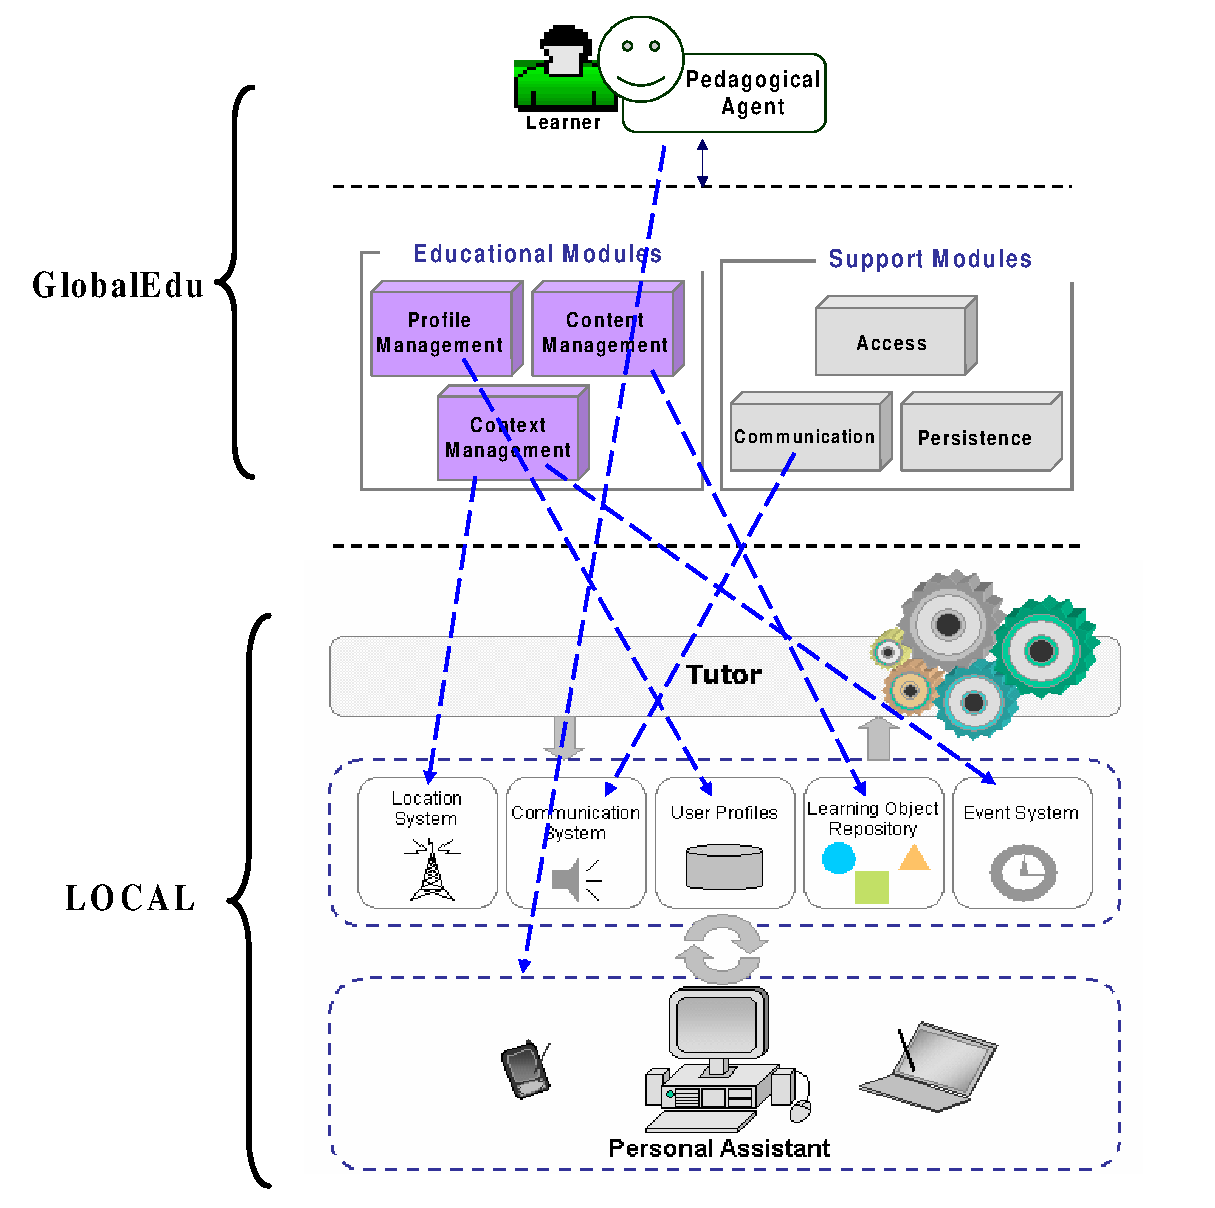
\includegraphics[width=0.5\textwidth]{media/local-ge}
  \caption{LOCAL adapted for GlobalEdu} 
  \label{fig:local-ge} 
\end{figure}
  
LOCAL is oriented to small-scale ubiquitous environments and its architecture
was projected to a centralized execution (only one server). As such, there is
only one GlobalEdu instance (see Figure~\ref{fig:ge-arch}). Modules are
executed in the network server and the PA executes in the users' mobile
devices.

%
% Practical scenario: GlobalEdu and LOCAL
%
\section{Practical scenario: GlobalEdu and LOCAL} \label{sec:scenario}

Our first choice in order to evaluate our proposal was the creation of a
small-scale ubiquitous learning scenario. We used the integration
GlobalEdu/LOCAL described in the section~\ref{sec:ge-local}. The prototype
scenario encloses nine rooms, covered by four wireless access points (see
Figure\ref{fig:scenario}). The location system has two parts: (1)~a webservice
created in C\# and~(2)~a database which stores context information. The
Personal Assistant was developed in C\#, using the .NET Compact Framework. The
assistant runs in iPAQs hx4700 and tablet PCs tc1100. It reads potency
information from the four wireless access points and forwards it to the
location system. The system uses this information to determine the position of
users' mobile devices. The profile system was implemented using MySQL. The
tutor and message system were also implemented as web services in C\#.

\begin{figure}[h!] 
  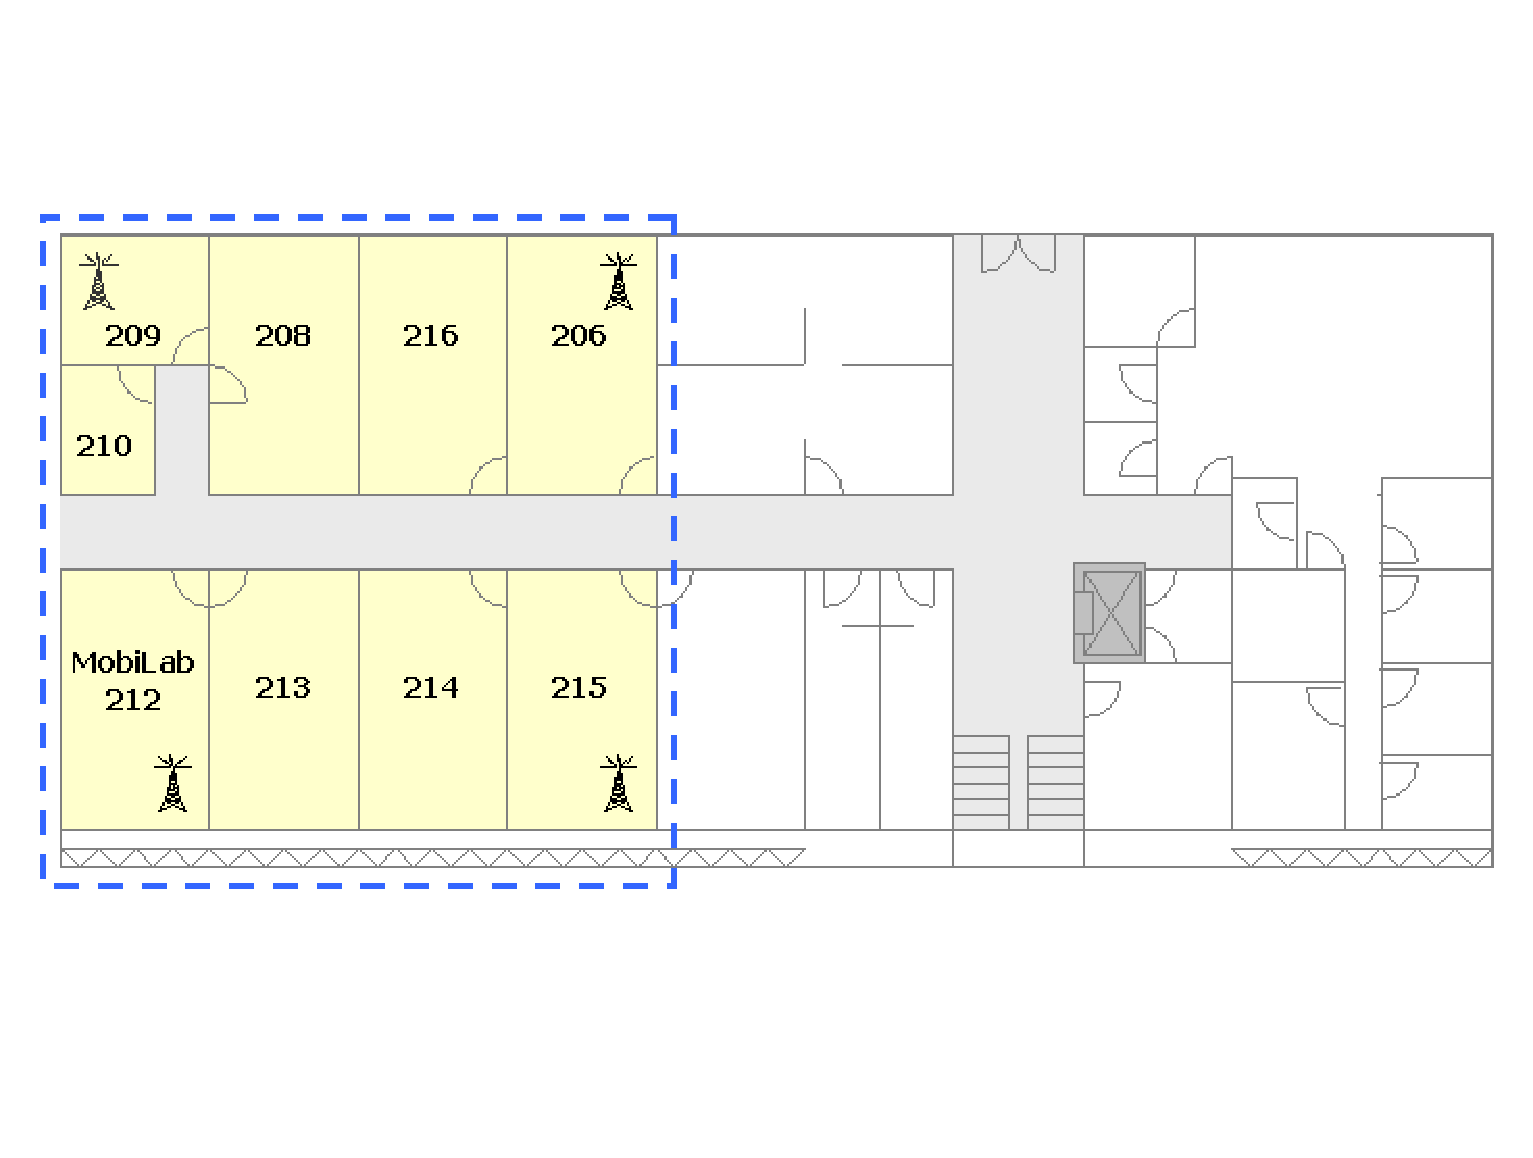
\includegraphics[width=0.5\textwidth]{media/scenario}
  \caption{Prototype Scenario} 
  \label{fig:scenario} 
\end{figure}

\subsection{Functionality Test 1: Following a Lession} \label{sec:test1}

The first moment occurs before the lesson. The professor sets an appointment
consisting of a message with the subject of the upcoming debate, as well as a
list of online resources. This appointment spans the whole duration of the
lesson. This message is tied to room 216, where the debate will occur. The
second moment corresponds to the start of the lesson. Seven students enter the
classroom, and are promptly detected by the location system. They receive the
appointed message. In the third moment, the professor requests the formation of
groups for debating. The groups are formed according with similarity between
user interests for ``Programming Languages''. In this particular case, three
groups were formed: one (A)~with four students interested in Java; the second
(B)~with two students interested in C\# and another one (C)~with just one
student, interested in C++. The debate starts, where each group presents the
pros and cons of each language. At this time, two students come late. Both
receive the appointed message, and are also informed about what group they
should participate in. One enters group A, and the other one enters group C. In
the fourth moment, another late student arrives, and receives the appointed
messages. However, the debate had already ended, and he is not directed to any
group. The fifth moment occurs after the ending of the lesson. The system
registers student attendance via sampled location data. A student is considered
present if he was in the classroom for at least 60\% of the meeting's duration.
The last student was considered absent.

\begin{table}
  \footnotesize
  \begin{tabular}{p{0.12cm}p{0.45cm}p{0.45cm}p{1cm}p{5cm}}
    \toprule
    & Initial Time & Final Time & Actor & Action \\
    \midrule
    \textbf{1} & - & 07:00 & Professor & Inserts an appointment, to be sent between 7:30 and 10:00, to all users in room 216. \\
    \midrule
    \textbf{2} & 07:30 & 08:00 & Learners & 7 users enter the room (authentication). \\
    \cmidrule(r){2-5}
    & 07:30 & 08:00 & System & Begins tracking the 7 users location. \\
    \cmidrule(r){2-5}
    & 07:30 & 08:00 & System & Message system sends the previously appointed message to all users in room 216. \\
    \midrule
    \textbf{3} & 08:00 & 08:10 & Professor & Solicits the creation groups for the debate. \\
    \cmidrule(r){2-5}
    & 08:10 & 08:10 & System & Sends messages, creates groups: A (4 users, Java), B (2 users, C\#) and C (1 user, C++). \\  
    \cmidrule(r){2-5}
    & 08:10 & 08:30 & Learners & The debate starts. \\
    \cmidrule(r){2-5}
    & 08:30 & 08:30 & Learners & 2 users enter the room (authentication).  \\
    \cmidrule(r){2-5}
    & 08:30 & 08:30 & System & Begins tracking position of the last 2 users. Sends appointed message to these 2 users. Informs where they should participate. \\  
    \cmidrule(r){2-5}
    & 08:30 & 09:00 & Learners & The debate comes to a conclusion. \\
    \midrule
    \textbf{4} & 09:00 & 09:10 & Learner & The last user arrives (authentication). \\  
    \cmidrule(r){2-5}
    & 09:10 & 09:10 & System & Begins tracking the last user position. \\
    \bottomrule
  \end{tabular}
  \caption{Simulated test}
  \label{tab:simulated}
\end{table}

The initial technological results proved that it was possible to: (1)~create
groups of students via profile and physical location data; (2)~distribute
material based on their profiles and in the debate theme; (3)~automatically
handle student attendances in the classroom, based on location data.

The previous simulated test couldn't present evidence of usability in a real
environment. In order to validate ubiquitous learning using GlobalEdu/LOCAL,
another experiment was conducted. This new experiment involved a sample
consisting of 20 individuals, between learners and professors of a Computer
Engineering undergraduate course at University of Vale do Rio dos Sinos
(Unisinos, Brazil).

This test was realized into five moments: each moment, a set of four
individuals interacted with the system. The following steps were considered:
1)~each participant was given an HP iPAQ hx4700 mobile device, which they used
to authenticate into the system; 2)~the participants then received suggestions
to participate in one of two workshops (based into user profile data); 3)~the
participants were notified whenever a professor they wanted to chat with was
available; 4)~in the fourth step, the system searched for matches between
participants' profiles, suggesting learning resources related to their
interests; 5)~the users were instructed to go to the workshop rooms. The
ubiquitous system then made available on the iPAQs the program of the chosen
event (per user). 

\subsubsection{Survey}

After following these steps, the users were asked to answer a survey, with
questions relating to their experience. The questions had answers in a scale
going from 1 (very weak) to 5 (excellent). An answer with the value 0 (zero)
meant the user had no particular opinion about that feature. The relation of
questions in the survey presented to participants is seen in
Table~\ref{tab:questions}. Several considerations can be made from the analysis
of each question. In order to demonstrate this, we have chosen charts
representative of the most important questions. 

\begin{table}
  \footnotesize
  \begin{tabular}{cp{7.5cm}}
    \toprule
    \# & ``What was your evaluation of\ldots'' \\
    \midrule
     1 & \ldots{}notifications about the availability of professors? \\ 
     2 & \ldots{}notifications about events, based on location and your profile data? \\
     3 & \ldots{}notification about the availability of physical resources? \\
     4 & \ldots{}information about users related to your interests, at your location? \\
     5 & \ldots{}the presentation of content related to events at your location? \\
     6 & \ldots{}the usefulness of this system for teaching? \\
     7 & \ldots{}the use of this system to determine your physical location? \\
     8 & \ldots{}the stimulus to interaction between users in the same location? \\
     9 & \ldots{}the possibility of using this system in daily activities? \\
    10 & \ldots{}the possibility of using this system in the classroom? \\  
    \bottomrule
  \end{tabular}
  \caption{Relation of questions}
  \label{tab:questions}
\end{table}


The aspects of context-awareness were analyzed through questions 1~to~7. There
was special interest into the adequate presentation of content related to
pedagogical events, and the use of the system to track user location.
Figure~\ref{fig:context} presents the results of these questions, as answered
by 20 test subjects. As can be seen, results indicate good acceptance in
relation to contextual information. 

\begin{figure}[h!] 
  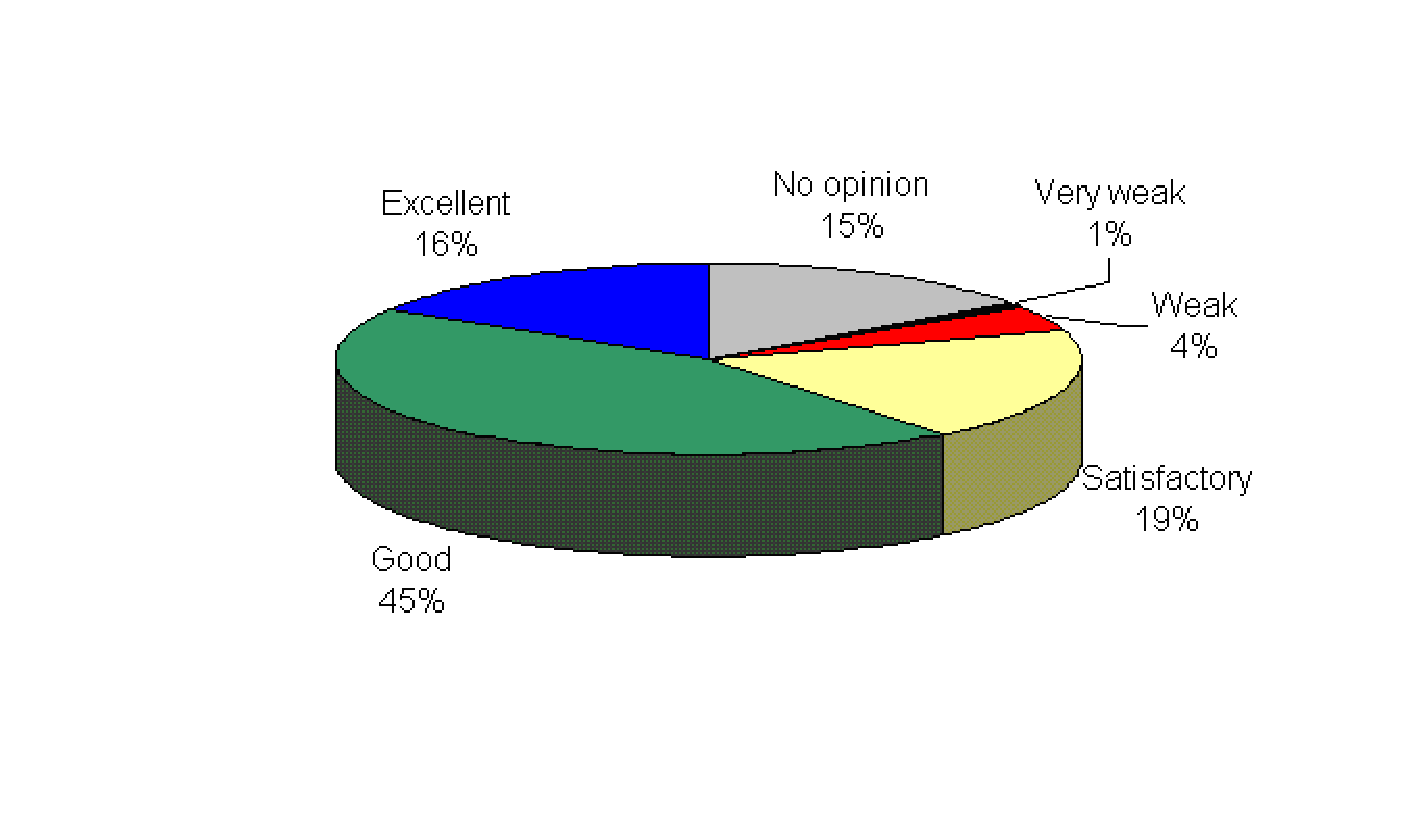
\includegraphics[width=0.5\textwidth]{media/context}
  \caption{Context data (questions 1 to 7)} 
  \label{fig:context} 
\end{figure}

The proposed daily use of the system as learning tool in the classroom, as well
as interaction between users and contextual elements were analyzed through
questions 8 to 10. These relate mostly to the usability of the system. The
results in Figure~\ref{fig:daily} indicate a good acceptance by the test
subjects. Over 60\% of those subjects considered the system \emph{good} or
\emph{excellent}. If we take into consideration the test was performed in a
limited and controlled scenario, the 32\% of people that considered the system
\emph{satisfactory} are also a good indication that this system is well fit for
daily usage. 

It should be noted that, in this survey, adaptability aspects were not given a
proper analysis. These aspects could be better analyzed if the test involved an
heterogeneous sample of mobile devices (desktop PCs, tablet PCs and iPAQs).

\begin{figure}[h!] 
  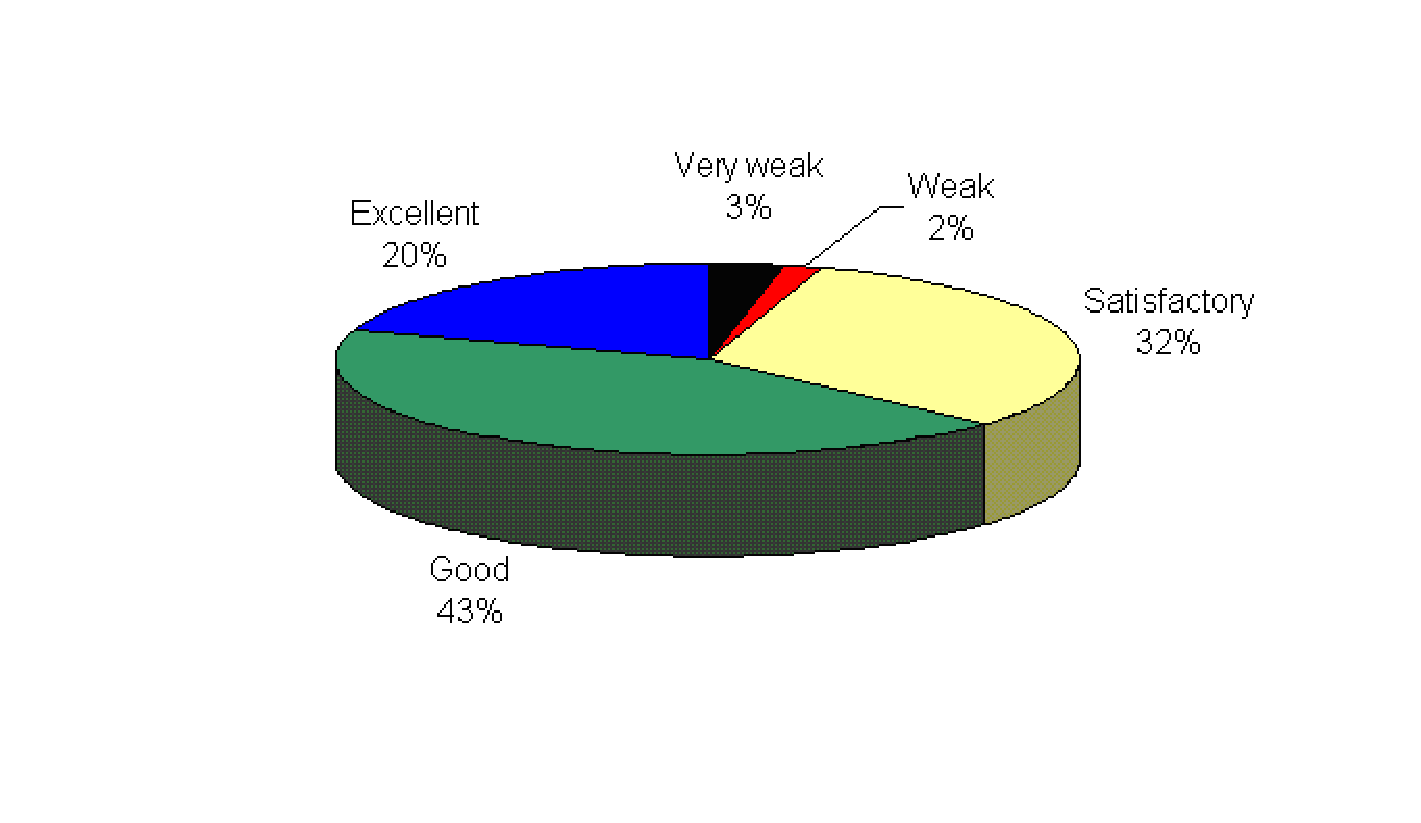
\includegraphics[width=0.5\textwidth]{media/daily}
  \caption{Daily usage (questions 8 to 10)} 
  \label{fig:daily} 
\end{figure}


\subsection{Functionality Test 2: Distributing Learning Objects}

The scientific community has been using scenarios to validate context-aware
environments (according to \citet{dey2001}'s approach) and ubiquitous
environments (according to \citet{satyanarayanan01}). Following this strategy,
our second experiment was a scenario involving the content distribution in a
daily routine of a Computer Engineering student.

This scenario focuses on the distribution of Learning Objects (LOs) in
different contexts based on the learner’s profile, according to the described
below:

\begin{quotation}
``Jorge is professor of the Programming Techniques discipline of the Computer
Engineering course at Unisinos. At the beginning of the week scheduled to the
basic teaching of programming using the Java language, he registered in the
LOCAL repository a group of learning objects (LOs) that support different
preferences of media (for example, text, video, and audio). The register
involved the indication of the contexts in which the objects would be
available.

In the classroom, Jorge registered some curricular objects concerning the basic
concepts. In the laboratory, he registered optional objects that will be
available for improvement, involving different themes (such as ``Interfaces''
and ``Parallel Programming''). 

João is a Computer Engineering student. At the day of the Programming
Techniques class, João entered the classroom and logged in the LOCAL using the
\emph{Personal Assistant} (see Figure 7(a)), subsequently he received a
notification of the availability of a curricular LO. João accessed the object
and received a PDF file (preference text). LOCAL used the \emph{Learner
Profiles} subsystem to determine this preference. 

After the class, João entered the laboratory and received a notification
regarding the availability of a LO related to the subject of his interest in
Java (in this case, ``Interfaces''). 

In the laboratory, João preferred audio objects, because he could listen to
them while he was using the computer (determined using the \emph{Learner
Profiles}).  João accessed the object and, after its use, received another
notification of available object (see Figure 7(b)) concerning the subject of
his interest (this time, the object was about ``Parallel Programming'').

Always that the students receive a notification of LOs, they can delay the
access. This action indicates that the students are interested in the object,
but they do not want to access it at the moment, i.e., they want to access the
object at the first opportunity of available time. João postponed the access to
the optional object (see Figure 7(c)).

At the end of the day, João moved to the train station. When he entered the
train, LOCAL notified him that a postponed LO was identified (Figure 7(d)).
Getting home, João still received another notification saying that the
professor had provided an additional object to a subject of his interest
(``Polymorphism'' in Java). In the register, the professor informed that the
interested students should be notified independently of their locations.''
\end{quotation}

The scenario was tested in the validation environment described in
Section~\ref{sec:test1}. The João student carrying an iPAQ 4700 simulated
the scenario, moving around the environment rooms. The train and the learner’s
house were simulated through the rooms 206 and 215.
Table~\ref{tab:distributing} summaries the actions, emphasizing the character
involved in each one. 

The results of this test proved that it was possible: 

\begin{enumerate}
  \item To distribute the learning objects using the contexts visited by the
        learners; 
  \item To use the learner’s profiles to choose the learning objects to
        be distributed; 
  \item To manage the access to the learning objects using the
        concept of postponed objects.  
\end{enumerate}

\begin{table}[h!]
  \footnotesize
  \begin{tabular}{p{0.12cm}p{1cm}p{5.9cm}}
    \toprule
    \# & Actor & Action \\
    \midrule
    \textbf{1} & Professor & Registers the learning objects in LOCAL, relating them to contexts.\\
    \midrule
    \textbf{2} & Learner & Enters the classroom and logs in LOCAL using an iPAQ 4700; see Figure 7(a) \\
    \midrule
    \textbf{3} & LOCAL & LOCAL detects the entry of the learner into the classroom. Tutor uses the \emph{Learner Profiles} to determine the learner’s preference of media in the context. Subsequently, it requests the sending of a message about the LO available in the preferred media. \\
    \midrule
    \textbf{4} & Learner & Accesses the curricular object. \\
    \midrule
    \textbf{5} & Learner & Moves to the laboratory. \\
    \midrule
    \textbf{6} & LOCAL & \emph{Tutor} detects the entry of the learner into the laboratory (\emph{Location System}) and uses the \emph{Learning Objects Repository} to verify the available LOs, related to the student’s interest. \emph{Tutor} still uses the \emph{Learner Profiles} subsystem to define the learner’s preferred media in the context. Finally, \emph{Tutor} requests to the \emph{Communication} subsystem the sending of messages about the available LOs; see Figure 7(b). \\
    \midrule
    \textbf{7} & Learner & Uses the \emph{Personal Assistant} to access one of the two identified objects and postpones the access to the other to the first moment of available time (see Figure 7(c)). \\
    \midrule
    \textbf{8} & Learner & Moves to the train. \\
    \midrule
    \textbf{9} & LOCAL & LOCAL detects the entry of the student into the train and calls the \emph{Learning Objects Repository} subsystem to verify the LOs that can be accessed during the trip. LOCAL identifies the postponed object and notifies the learner, see Figure 7(d). \\
    \midrule
    \textbf{10} & Learner & Accesses the object that has been postponed. \\
    \midrule
    \textbf{11} & Professor & Registers a new optional LO concerning ``Polymorphism'' in Java that can be accessed in any context. \\
    \midrule
    \textbf{12} & Learner & Enters his home. \\
    \midrule
    \textbf{13} & LOCAL & Tutor informs the learner (Communication subsystem) of the new optional LO available that corresponds to his areas of interest. \\
    \midrule
    \textbf{14} & LOCAL & Accesses the new object. \\
    \bottomrule
  \end{tabular}
  \caption{Distributing Learning Objects}
  \label{tab:distributing}
\end{table}


\section{Related work} \label{sec:related}

Some projects are investigating the use of ubiquitous computing to provide new
learning perspectives. \citet{ogata03} present JAPELAS, a context-aware system
to support learning of Japanese language expressions. Learners carrying PDAs
are assisted by the system to help identify the adequate polite expressions,
considering the context where they are. JAPELAS is directed for a specific
content. With GlobalEdu's \emph{Content} Management it's possible to learn
about any kind of content. 

The Ambient Wood Project \citep{rogers05} is dedicated to the design and
building of pervasive environments. WiFi and sensor-based technologies are
connected with a variety of mobile and standalone computational devices. The
proposal is that digital augmentation offers a promising way for enhancing both
indoors and outdoors learning processes. The GlobalEdu \emph{Context Managment}
module uses the Social and Physical information to improve the learning
process. LOCAL explores indoors learning applications through WiFi technology,
and with ISAM, we intend to explore both indoors and outdoors applications.

A ubiquitous computing scenario needs to support general purpose educational
processes, where mobility, context and learner information will be considered.
None of the current projects \citep{rogers05,ogata03} addressing this
particular problem use location data to both: (a)~accurately track users'
movements; (b)~present contextual information to the learner. As such,
GlobalEdu (alongside LOCAL) presents an innovation in this aspect, since
location data can be used in many new pedagogical opportunities.


\section{Conclusion} \label{sec:conclusion}

GlobalEdu is an innovative proposal that allows the exploration of the benefits
of ubiquitous learning environments. Different from other approaches, GlobalEdu
does not depend on a specific ubiquitous environment. Also, it can be coupled
with mostly any learner model or learning objects model. 

The results of the experiments show that GlobalEdu can be used in a specific
classroom learning situation and in generic learning situations. Currently, we
are improving the GlobalEdu prototype and its integration with LOCAL. After
that, another round of tests shall be conducted.

%
% Bibliografia
%
\bibliographystyle{plainnat} 
\bibliography{globaledu_local}


\end{document}
